\chapter{A Method for Performance Testing Distributed Middleware Based Systems}
\label{Chapter:Methodology}

Size and complexity of software systems are increasing and there is increasing demand for component based distributed applications and systems. Performance characteristics such as throughput and scalability are crucial quality attributes of such systems. For this reason, it is very critical to validate that the system satisfies the performance requirements. Performance testing is a way to evaluate performance characteristics. 

This chapter will introduce a method to help build a distributed middleware based system, capture its performance characteristics and perform performance testing and/or performance engineering on it. The method consists of creating a domain specific modeling language for capturing the structure and performance characteristics of the system, and creating a discrete event based system model to capture the behavior of the system. 

The domain specific modeling language is created by using the concepts and tools introduced by Model Integrated Computing (MIC). A brief background on MIC will be given in the following sections in this chapter. The behavioral model is created by Discrete Event System Specification (DEVS) which is a modeling and analysis formalism for discrete event systems \cite{Zeigler84}. A background of DEVS is given in Chapter \ref{Chapter:DEVS}. 


\section{Challenges of Performance Testing Distributed Middleware Based Systems}

Distributed systems are generally built on top of middleware platforms. Primary goal of middleware is to provide the means for components to connect and interact with each other and the underlying operating system and network protocols. Furthermore, middleware aims to make the integration of heterogeneous components easier \cite{SS01}. Large scale distributed systems generally have stringent performance requirements. Throughput, latency, scalability are important performance metrics for such systems \cite{Weyuker00, Gao03}. For this reason, performance testing plays an important role in middleware based distributed systems. 

Middleware platform provides services such as transactions, and remote communication which affect the performance of a system in a big way. The role of middleware often makes it the entity that is most influential on the overall performance of the system \cite{LiuGorton02}. Although the big effect of middleware on the whole system performance cannot be denied, it is also important to consider the relationships of the components with each other and the middleware when performance testing a system. Moreover, it is important to take into account the context of the distributed application since a middleware may behave differently in different contexts \cite{Denaro04, Denaro05}. Tight coupling between the components and the middleware would potentially cause complex component interactions. Those complex interactions would potentially affect the performance of the system. As components cannot be executed without the underlying middleware system, it is not sufficient to perform performance testing on the components in isolation in order to understand the performance of the system. Likewise, performance testing middleware in isolation would not be enough because coupling with the components that use its services is too important to ignore. 

An aspect of testing a high performance distributed middleware framework and its components is creating many configurations that would configure functional operation of components as well as their deployment in the cluster. The configurations are usually described by XML. It is cumbersome and inefficient for test engineers to write XML test configurations by hand as the tester would be making many copy-paste operations which can introduce errors into the process. Moreover, the configuration space of the control and deployment parameters of applications within the framework is sufficiently large; there is no way for the tester to manually create configurations for all possible combinations of parameters. Last but not the least, it would be very time consuming to scale up and modify a manually written XML test configuration in response to changes in hardware resources or other test criteria.

In the following section, an approach based on model based testing and test generation will be described.

\section{A Model Based Approach to Performance Testing Distributed Systems}
\label{Section:TSDML}

In the previous section, several challenges for performance testing a distributed middleware based system was given. As a result of a literature review on the subject matter \cite{areapaper} the following observation was made: \textit{There is a need for a way to characterize and capture performance characteristics of components and the component model in a distributed system. Such a model would help explore the effect of complex component interactions on system performance. In order to be able to test the performance of the system by taking into account the couplings of components and middleware, component interactions should precisely be understood and captured from a performance perspective in a component oriented performance model. Such a performance model can be used to automatically generate executable performance test cases.} 

A systematic modeling approach for characterizing and capturing distributed system components' and underlying middleware's performance properties can be used to tackle the challenges described above. The systematic modeling can also be used to investigate the effects of different component-component and component-middleware interactions on the performance of the system. 

The systematic modeling approach which is described in this chapter uses a two layered modeling approach. One layer of modeling is done using a model based design methodology called Model Integrated Computing (MIC) \cite{Greenfield2004Software, MIC}. The second layer of modeling is done using the Discrete Event System (DEVS) Specification modeling and analysis formalism for discrete event systems which is described in Chapter \ref{chapter:DEVS}. 

As a model based design methodology, MIC provides a scalable methodology for system design and analysis based on sound system theory and abstraction by integrating the efforts in system specification, design, synthesis, validation, verification and design evolution. MIC brings in key concepts of domain modeling to the paradigm of model driven system development. A key capability supported by MIC is the definition and implementation of domain-specific modeling languages (DSMLs). Crucial to the success of DSMLs is metamodeling and auto-generation. A metamodel defines the elements of a DSML, which is tailored to a particular domain. The modeling language which is used to construct metamodels is known as a metamodeling language. Auto-generation involves automatically synthesizing useful artifacts from models, thereby relieving DSML users from the specifics of the artifacts themselves, including their format, syntax, or semantics.

The properties of the MIC methodology provides a strong means to tackle challenges mentioned above. Using MIC and its accompanying tool Generic Modeling Environment \cite{GME} enables the creation of a DSML targeted for distributed middleware based systems and enables incorporating performance testing aspects. Furthermore, auto-generation capabilities of GME enables synthesis of series of configurations and tests. On the other hand, DEVS modeling formalism enables modeling the behavior of MIC model components and provides a event based simulation engine for easily observing the effect of changes in behavior in the performance of the system.


The following steps are involved in using the model based approach that is described in this chapter:

\begin{itemize}
	\item Identify the applications (including the middleware) of the system and their configuration parameters
	\item Identify the relationships and interactions between applications
	\item Identify the structure and data flow in the system
	\item Identify the behavior of each application in the system
	\item Identify the physical (processor, network card) and logical (ports) resources that will be needed in the system
	\item Model identified applications, their relationships, and resources using the Test Series Definition Modeling Language (TSDML)
	\item Model the behavior of of the applications and the event based data flow using DEVS modeling formalism
	\item Identify performance metrics for the applications and the system
	\item Configure the DEVS behavioral model with the information captured in TSDML
	\item Run the DEVS simulator to collect performance results
	\item Alternatively, run the system with the configuration generated from the TSDML
\end{itemize}

****TODO: add the high level diagram of the approach here****

In the following section, the domain specific modeling language called Test Series Definition Modeling Language (TSDML) will be described in detail.

\subsection {Test Series Definition Modeling Language}

Test Series Definition Modeling Language (TSDML) is a domain specific modeling language designed to model distributed component based systems from a performance testing point of view. TSDML aims to make it easier to capture the structure and interaction of components along with the performance characteristics of the system. 

The TSDML has the following high level properties:

\begin{itemize}
	\item Define application types
	\item Define the connection association between applications by connection rules
	\item Define association rules between applications and contexts
	\item Define association rules between connections and logical networks
	\item Define association rules between context and hosts
	\item Define replication factors for the types and connections
	\item Form a template test case from the modeled applications, connections, and resources
	\item Define the scope of the test series
\end{itemize}


In the following sections details of the modeling process and abstraction levels for these aspects will be described. 

\subsubsection{Modeling Application Types}
An important advantage of using MIC model based methodology is the ability to view the system to be modeled from different aspects and enable separation of design concerns. From this perspective TSDML defines two different aspects for modeling an application (type): Data Flow Aspect and Test Definition Aspect.

From the Data Flow Aspect an application is modeled to contain Parameters, Input Data Port, Output Data Port, and Bidirectional Data Port. From the Test Definition Aspect an application is modeled to contain Sweeper (see Subsection \ref{SubSubSection:Parameterizing}), Negative Probe, Positive Probe and reference to Iterator (see Subsection \ref{SubSubSection:Parameterizing}). The application metamodel is shown in Figure \ref{fig:ApplicationMetaModel}.

\begin{figure}
	\centering
		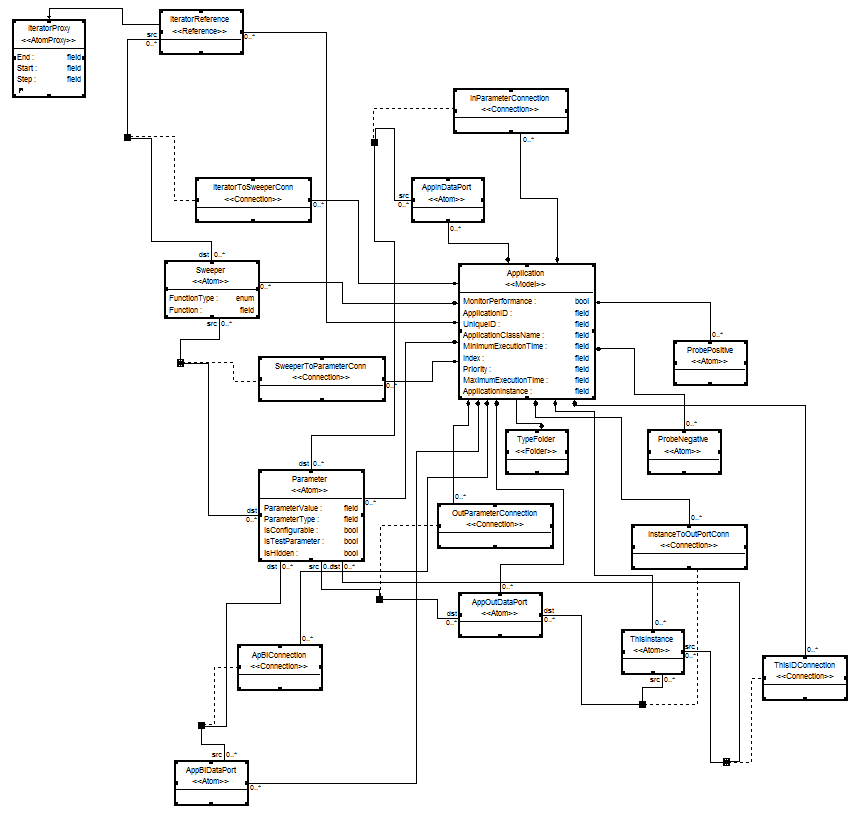
\includegraphics[width=0.60\textwidth]{figures/ApplicationMetaModel.png}
	\caption{Application metamodel in GME}
	\label{fig:ApplicationMetaModel}
\end{figure}

The Data Flow Aspect lays out the data ports that the application has and the parameters to configure the application. The data ports can be input only, output only and bidirectional. The application has the following attributes:

\begin{itemize}
	\item MonitorPerformance: Boolean flag to denote whether the performance of the application needs to be monitored
	\item ApplicationID: Unique identification number of application
	\item ApplicationClassName: Class name of the application's implementation
	\item MinimumExecutionTime: Minimum execution time of the application
	\item MaximumExecutionTime: Maximum execution time of the application
\end{itemize}

The parameters of the application have the following properties:

\begin{itemize}
	\item ParameterValue: Value of the application parameter
	\item ParameterType: Basic type of the application parameter (e.g. double, int)
	\item IsConfigurable: Boolean flag to denote if the parameter is a configurable parameter
	\item IsTestParameter: Boolean flag to denote if the parameter is a test parameter
\end{itemize}

The Test Definition Aspect provides Sweeper to vary the values of test parameters of an application and Negative Probe and Positive Probe to attach performance measurement points.

Sweeper is an important element in TSDML which has the following attributes:

\begin{itemize}
	\item Function Type: Internal function or look-up table. Internal function is a function of test series iterator whereas the look-up table may have specific values that an application can take.
	\item Function: The definition of the function.
\end{itemize}

Sweeper is attached to an application parameter and varies the value of the parameter based on the function provided in its attribute. A new value for an application parameter is used in each test case that will be generated from the model.

Figure \ref{fig:ApplicationModelDataFlow} shows the Data Flow and Figure \ref{fig:ApplicationModelTestSeries} shows the Test Series Definition aspect of sample application model.

\begin{figure}
	\centering
		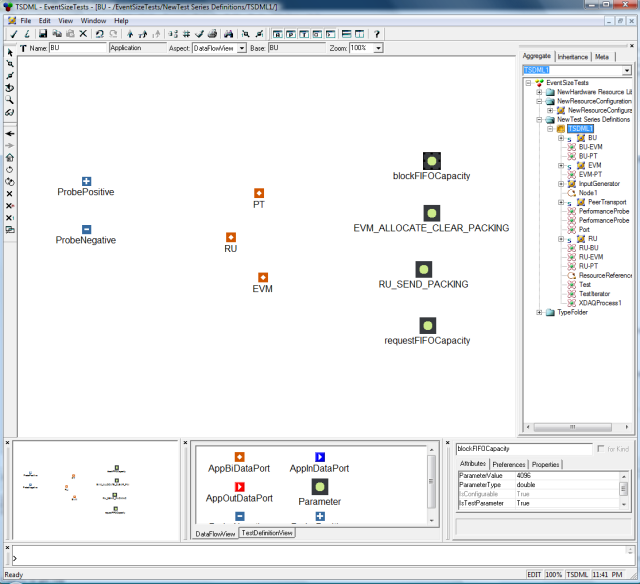
\includegraphics[width=0.60\textwidth]{figures/ApplicationModelDataFlow.png}
	\caption{Data Flow Aspect of a Sample Application Model}
	\label{fig:ApplicationModelDataFlow}
\end{figure}

\begin{figure}
	\centering
		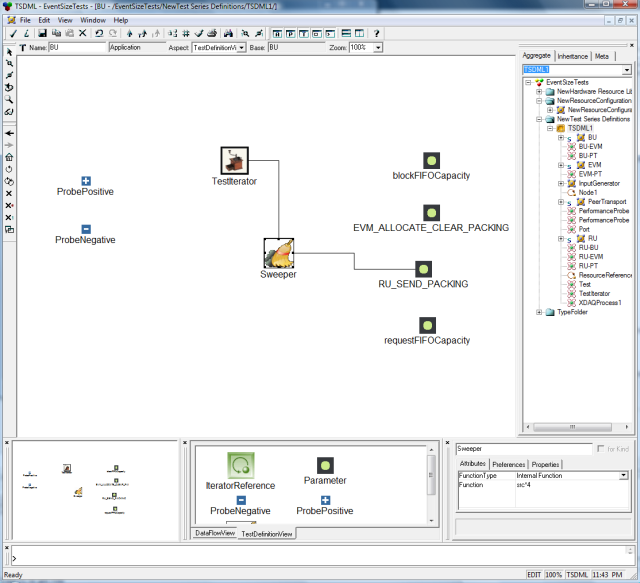
\includegraphics[width=0.60\textwidth]{figures/ApplicationModelTestSeries.png}
	\caption{Test Series Definition Aspect of a Sample Application Model}
	\label{fig:ApplicationModelTestSeries}
\end{figure}

Modeling application types in this manner tackles several challenges mentioned in the previous sections. This approach treats both the middleware and its applications as application types and enables modeling and configuration of them separately. For this reason, it will be possible to consider not only middleware-application relationships but also application-application relationships. In addition, it'll be possible to identify the couplings between middleware and applications that use its services.

****TODO: Change figures to metamodel figures. Will use the model figures in the implementation****

\subsubsection{Modeling Resources and Resource Configurations}
TSDML includes a way to model the resources to be used to deploy the system. A simple abstraction has been chosen for TSDML for modeling resources. However, it can easily be extended to drill down to the details of resources and resource management. Two main parts are the resource library and the resource configurations. TSDML has been constructed such that resource library collects models of the resources that can be used in a resource configuration. Resource configurations use references to resource models in the library to define specific configurations.

Resource is described as a \textit{Node} in TSDML. TSDML uses the following entities and their attributes to define a node:

\begin{itemize}
	\item Network Card (NIC)
	\subitem IP Address
	\subitem Network Type (e.g. Gigabit, Infiniband, etc.)
	\item Processor
	\subitem IP Address
\end{itemize}

\begin{figure}
	\centering
		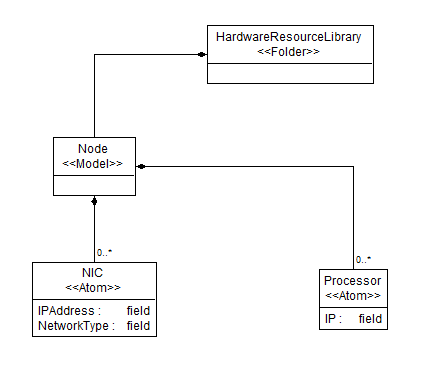
\includegraphics[width=0.60\textwidth]{figures/ResourceLibraryMeta.png}
	\caption{Resource Library Metamodel}
	\label{fig:ResourceLibraryMeta}
\end{figure}


Resource configuration model is described by a reference to a node that is created in the resource library model. The main point of a resource configuration model is to define the connections between the nodes. A connection between nodes is made through the \textit{Network} entity. TSDML uses the following entities and their attributes to define a resource configuration:

\begin{itemize}
	\item Node Reference: Reference to a node created in resource library
	\item Network
	\subitem Network Type (e.g. Gigabit, Infiniband, etc.)
\end{itemize}

\begin{figure}
	\centering
		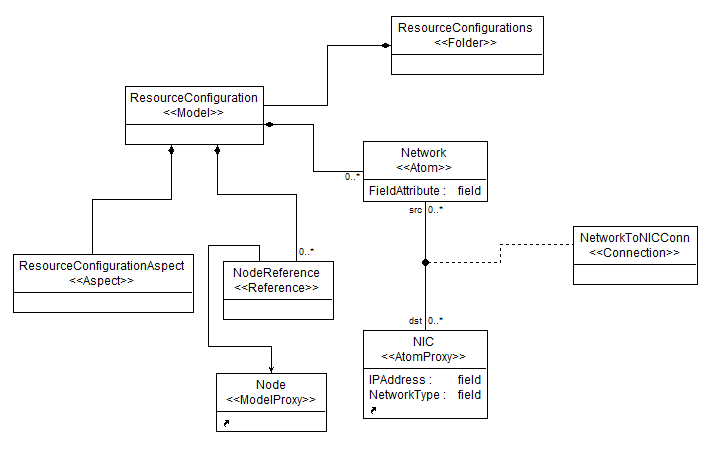
\includegraphics[width=0.60\textwidth]{figures/ResourceConfigMeta.png}
	\caption{Resource Configuration Metamodel}
	\label{fig:ResourceConfigMeta}
\end{figure}


\subsubsection{Parameterizing the Model}
\label{SubSubSection:Parameterizing}
As mentioned previously, it is desired that the TSDML model should be parametrized in order to be able to generate series of test cases from a single model. The parameterization is achieved by using ``Iterator'' and ``Replicator'' entities in the system model.

\textbf{Iterators} are used to define the series $i, j, k ...$ for the notions of $\left\{start, step, stop\right\}$. There can be many iterators in a test series definition.

\textbf{Replicators} are used to define the replication factor for the attached object. The replication factor determines how many of the object to which the replicator is attached to will be generated when the model is interpreted. Replicators are functions of iterators as in $r = K \times si$. There can be many replicators in a test series definition. Replicators must be attached to an iterator in the model since they are functions of iterators. They must also be attached to an application, network or context entity.

Figure \ref{fig:iterator-replicator} shows a possible example use of replicators and iterators in the model to generate multiple instances of two different application models. 

\begin{figure}
	\centering
		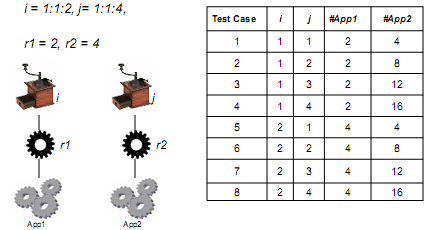
\includegraphics[width=0.90\textwidth]{figures/iterator-replicator.png}
	\caption{Use of iterators and replicators in the model}
	\label{fig:iterator-replicator}
\end{figure}

In the example, it is assumed that $i = 1:1:2$ and $j = 1:1:4$ and $r1 = 2$ and $r2=4$. By design, iterators function as the outer loop whereas the replicators function as inner loops. In this case, the table in Figure \ref{fig:iterator-replicator} shows the total number of test cases that will be generated and the numbers of App1 and App2 instances in those test cases. In this example, total of $8$ cases will be generated and number of App1 instances will change between $2$ and $4$ and the number of App2 instances will change between $4$ and $16$.

Iterators and connectors also function similarly when there is a connector between applications. Figure \ref{fig:iterator-connector} shows an example of such a situation. 

\begin{figure}
	\centering
		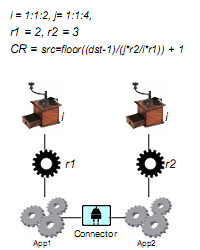
\includegraphics[width=0.40\textwidth]{figures/iterator-connector.png}
	\caption{Use of iterators and replicators with connectors}
	\label{fig:iterator-connector}
\end{figure}

\begin{figure}
	\centering
		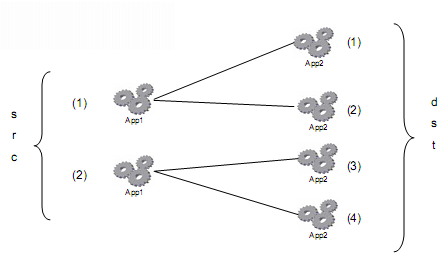
\includegraphics[width=0.80\textwidth]{figures/iterator-connector2.png}
	\caption{Resulting Configuration for Example 2}
	\label{fig:iterator-connector2}
\end{figure}

As described above, since connectors are boolean functions of iterators and replicators, it is possible to define the connection relation between applications with respect to the iterators and replicators to which the applications are attached to. In the example shown in Figure \ref{fig:iterator-connector}, iterator $i$ is defined as $i = 1:1:2$ and iterator $j$ is defined as $j = 1:1:4$ and replicators r1 and r2 are defined as $2$ and $3$ respectively. The connection relation between applications is defined as the boolean function $src = floor((dst-1)/(j \times r2 / i \times r1)) + 1$. As can be seen in the figure, App1 is the source (src) and App2 is the destination (dst). 

In order to fully understand what type of a model this example will lead to, we should first consider the iteration and replication of the applications. This example shares the same configuration for applications as shown in Figure \ref{iterator-replicator}. That is, there will be a total of 8 test cases. For the first test case, there will be 2 instances of App1 and 4 instances of App2. The connection between these applications is determined by the connection relation and results in the configuration shown in Figure \ref{iterator-connector2}. 

Modeling iterators and replicators as part of the TSDML aims to tackle the challenge of writing and managing many test configurations. By using iterators and replicators and taking advantage of auto generation capabilities of the modeling approach, a test engineer will be able to create and control many test cases with minimal effort. 

The concept of iterators and replicators easily and conveniently achieve the parameterization goal of the TSDML and enable creation of series of test cases from the single test template model. 

\subsubsection{Modeling Input Generator}
Input Generator is an important entity in the TSDML. It is not necessarily part of the overall system however it is crucial to model the input to the system for testing purposes.

In TSDML, input generator is modeled as a construct containing some parameters. The input generator is assumed to be used for generating events for the event based system. The following parameters make up the input generator:

\begin{itemize}
	\item Input Generator Parameter: Any parameter that may relate to modeling an input generator (e.g. mean, sigma, etc.)
	\item Random Distribution: Enumeration to model the type of distribution (e.g. Lognormal, normal, exponential, etc.)
	\item Parameter Sweeper: Similar to application types, a sweeper can be connected to parameters to vary the values of parameters for each test
	\item Iterator Reference: Reference to the iterator used for test series definition. 
\end{itemize}

Most important part of the input generator model is the parameter sweeper. It is the same sweeper that is used for varying values of application parameters. By connecting the iterator reference to a sweeper, values of input generator can be varied for each test case to be able to test the system against varying input data.

Based on the design of the system, the input generator can be connected to any application which accepts the input data and is the trigger for the operation of the system. Figure \ref{fig:InputGeneratorMetaModel} shows the Input Generator portion of the TSDML metamodel.

\begin{figure}[htb]
	\centering
		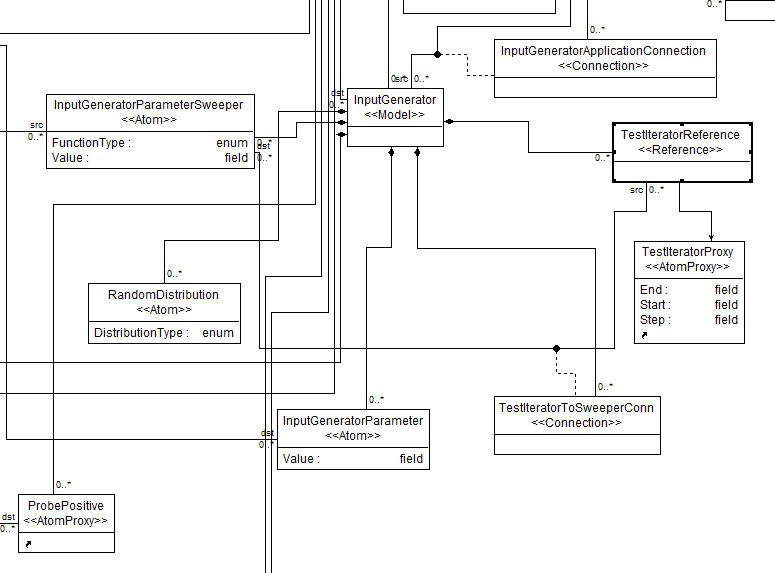
\includegraphics[width=0.70\textwidth]{figures/InputGeneratorMetaModel.PNG}
	\caption{Input Generator Meta Model}
	\label{fig:InputGeneratorMetaModel}
\end{figure}

\subsubsection{Modeling Test Series Definitions}

\begin{figure}[tbp]
	\centering
		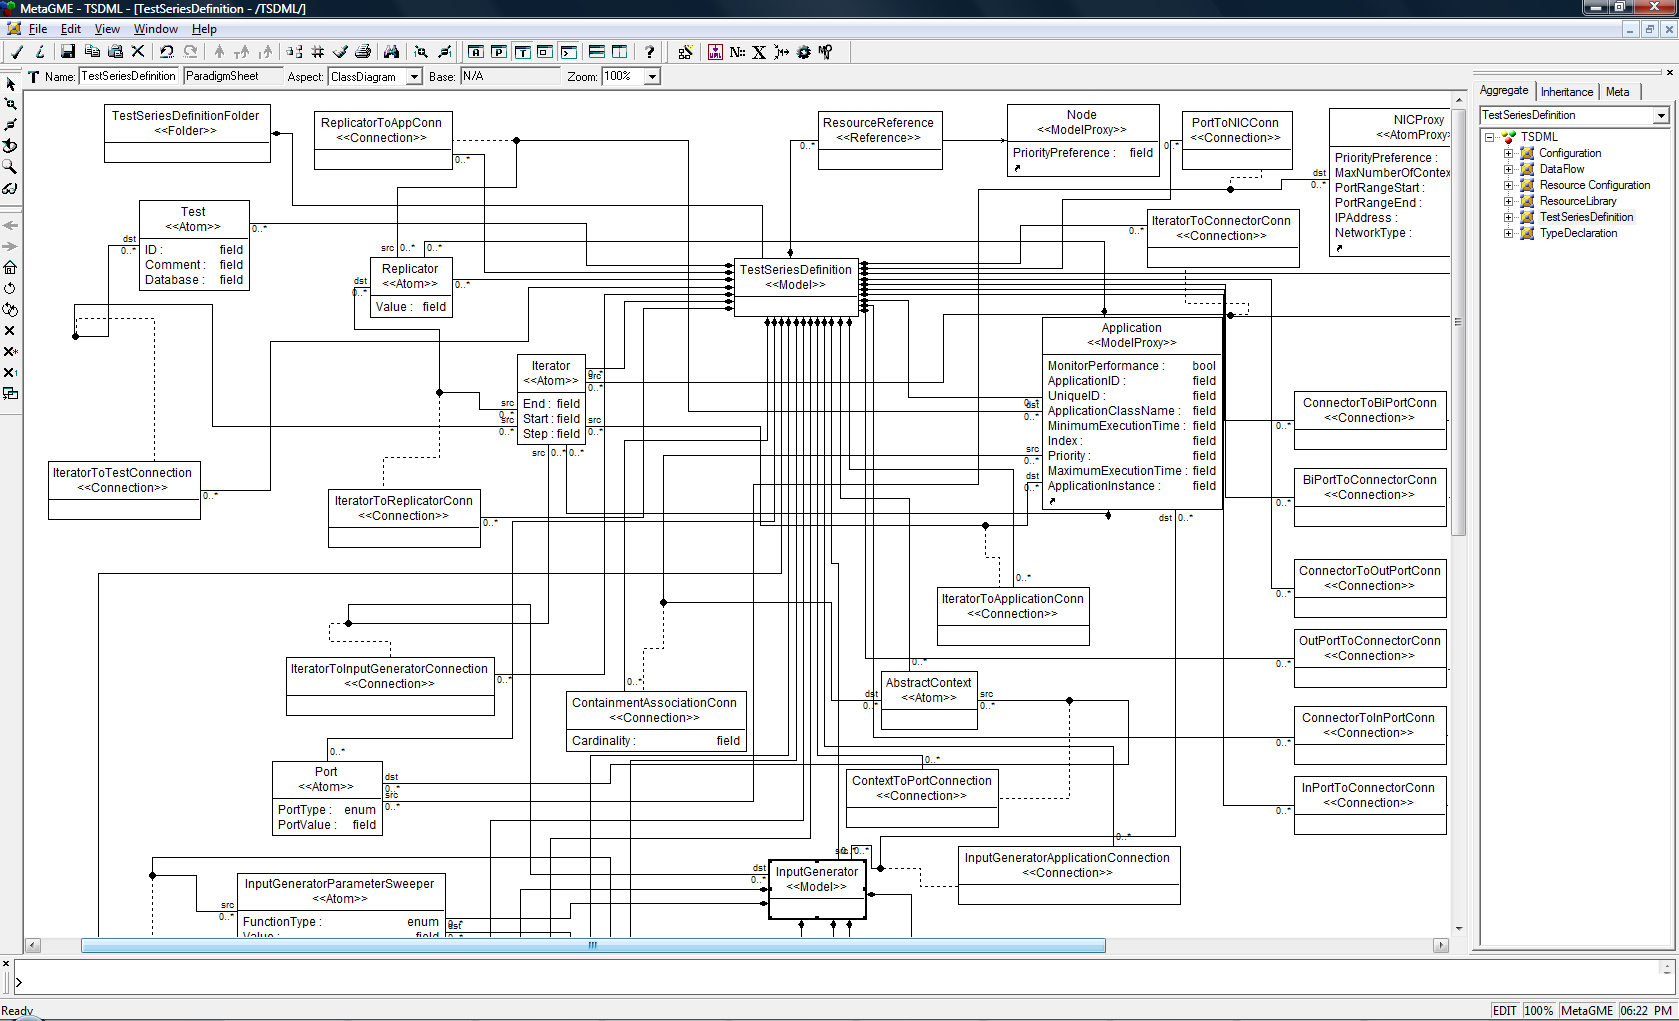
\includegraphics[width=0.90\textwidth]{figures/TestSeriesDefinition.png}
	\caption{Test Series Definition Meta Model}
	\label{fig:TestSeriesDefinition}
\end{figure}

Test series definition models bring together all the entities of the TSDML from a test generation perspective and enables generation of series of test cases utilizing model parametrization described in the previous subsection.

An important advantage of using MIC model based methodology is the ability to view the system to be modeled from different aspects and enable separation of design concerns. From this perspective TSDML defines three different aspects: Test Series Definition Aspect, Deployment Aspect, Performance Aspect. All there aspects of modeling a test series definition will be explained in detail.

The \textit{\textbf{Test Series Definition Aspect}} includes all the modeling elements that were described in the previous subsections. Test Series Definition aspect acts like a design surface for designing series of test cases. It contains the following modeling elements:

\begin{itemize}
	\item Application Reference
	\item Iterator
	\item Replicator
	\item Connector
	\item Input Generator
	\item Test entity
	\item Connections between these entities
\end{itemize}

References to application types and connectors that connect the applications make up the data flow among the applications. In order to create a test series definition not all application types need to be present. Different test series definitions with different applications and with same applications and different parameter values can be modeled since test series definitions are collected under a folder structure and lead to different set of test cases.

Iterators and replicators are the entities which define the scope of the series and add parameterization to the test series definition model. As described in "`Parameterizing the Model"', a replicator enables using a single application type and generate multiple application instances during test case generation. By use of replicators and iterators, it is possible to easily create a template of an application to be replicated at each step of test case generation.

Connector defines the relationship and data flow between the applications. When a connector entity is used to connect ports of two applications, it denotes that there is a data flow between those applications. As explained before, it is also a very powerful entity with its ConnectionRule property which is a function of the iterator. Making connections this way enables variations on the application structure that is to be tested.

The InputGenerator entity supplies the test data to the system to drive the test run. It can be connected to the applications which are expecting data to be enabled.

The Test entity is a placeholder entity which captures the general information about the test that is being designed. The information captured is used to store the results of the test run appropriately in a database or test log. The primary attributes of the Test entity are the Comment and Database fields. The Comment field is used to give a brief description of the test series being designed. The Database field is used to capture the name of the database that the test results will be saved to.

A test series definition is obtained when all these entities are connected to each other appropriately. The number of test cases that will be generated from one test series definition is based on the value of the iterator. 

The Test Series Definition aspect provides the solution for the challenge of manually creating several XML test configurations and makes the process easier to scale and less time consuming. In addition, by bringing together the pieces that are mentioned in the previous sections, this view makes it possible to span a considerable portion of the configuration space of parameter applications. This is made possible by being able to change application parameter values by means of Sweepers and control this change by iterators and replicators for each test case.

****TODO: May rewrite to better focus on answers to the challenges.****

The \textit{\textbf{Deployment Aspect}} includes modeling entities that can be used to devise different deployment scenarios for the system. The following entities can be used in this aspect:

\begin{itemize}
	\item Application (Reference)
	\item Resource (Reference)
	\item Middleware
	\item Port
\end{itemize}

Any common entities across aspects are carried over to the respective aspect. For this reason, the application reference is the same as the on used in the Test Series Definition aspect. The difference across different aspects is the perspective those entities are being looked at. While in the Test Series Definition aspect, the application reference was viewed from the perspective of creating a test series definition with multiple instances of applications generated automatically. In this aspect, the applications are viewed from a deployment perspective. The connections that are to and/or from an application reference are related to the deployment aspect of the system. 

Resource reference is a reference to any resource that is modeled in the Resources and Resource Configurations. Deployment aspect is the only place where a resource can be utilized because it's inherently related to deployment. From the testing perspective, having a resource model in this view makes it possible for a test designer to deploy a system on various resources and devise several test cases.

Another entity in the Deployment aspect is Middleware. It is a key entity for deployment because applications cannot run in absence of middleware and have to be deployed in a middleware instance. Technically, middleware is no different than an application, it's defined and modeled with application types. However, it's special in the sense that can contain other application types. As applications can be deployed on middleware, middleware is deployed on resources on specific ports.

Port, as the name suggests, is a logical entity used to define endpoint for the application on the resource that it is deployed to. It is used to connect middleware to a resource. Port has the following attributes:

\begin{itemize}
	\item Port Type: Type of port (e.g. TCP/IP, SOAP, etc.)
	\item Port Value: Value of port (e.g. 8080, 4000, etc.)
\end{itemize}

\textit{\textbf{The Performance Aspect}} includes entities related to capturing performance information about the system. The main entity of this aspect is the Performance Probe. It's designed to be analogous to a voltmeter or ammeter used to measure electric voltage and current in electronic circuits. In this manner, a performance probe is connected to positive and negative end points and measures a performance metric between those points.

A performance probe has one attribute:
\begin{itemize}
	\item Metric: It's an enumeration of possible performance metrics to be measured (e.g. throughput, latency, bandwidth).
\end{itemize}

For example, when a performance probe is connected between the negative probe end of App1 and positive probe end of App2 and its metric is set as Throughput, it means that throughput between App2 and App1 will be measured.

All the aspects of the Test Series Definition make up the main parts of the TSDML. Test series definition uses the modeling constructs defined elsewhere to model a system from test, deployment and performance points of views. 

\subsection{Modeling Behavior with DEVS}
The Test Series Definition Modeling Language makes it possible to model the system from various perspectives. It is a graphical domain specific language that can be used to capture structure and data flow of a system from a higher level of abstraction. TSDML also enables the design of a system from the testing perspective. 

In model driven engineering, the crucial step after modeling a component or a system is to be able to interpret the meaning of the abstractions in the model. The artifact of such interpretation can be a design document, source code, etc. In the case of the approach described in this chapter and the TSDML, the desired artifact is several test cases (e.g. in the form of XML configurations) that can be executed on the real implemented system. 

In some cases, the real implementation of the system modeled by TSDML may not be available. Moreover, it may not always be feasible to execute the test cases on the real system. An implementation of the system may not yet be available or it may be costly to run unpredictable tests on the real implementation or replicate the real system setup for testing purposes. In such cases, it is important to be able to model the behavior of the system as well. 

In the approach described in this chapter, the behavior model of the applications of the system is created using the Open DEVS modeling formalism. A background on Open DEVS is given in Chapter \ref{Chapter:DEVS}. 

DEVS modeling formalism and the underlying simulation framework enables the execution of test cases generated from TSDML on a simulated system. In order to achieve that, each application type that is modeled using TSDML should have a corresponding DEVS behavior model. An application is modeled using DEVS as described in Chapter \ref{Chapter:DEVS}. The main aspect of this process is correctly determining:

\begin{itemize}
	\item States of the application
	\item Input and output events of the application
	\item Input and output connections/ports of the application
\end{itemize}

Since DEVS is an event based framework, it is possible model the data flow and interactions among applications. In a middleware based system, it is particularly important to determine interactions between applications. It is possible with DEVS to model the application interaction in such a way that no application can talk to each other without going through middleware. 

An example implementation of a DEVS model will be given in Chapter \ref{Chapter:Implementation}.

\section{Closing the Loop: Performance Engineering}
Size and complexity of software systems are increasing and there is increasing demand for component based distributed applications and systems. Performance characteristics such as throughput and scalability are crucial quality attributes of such systems. For this reason, it is very critical to validate that the system satisfies the performance requirements. Performance testing is a way to evaluate performance characteristics. 

IEEE Standard Glossary of Software Engineering Terminology defines performance testing as ``testing conducted to evaluate the compliance of a system or component with specified performance requirements'' \cite{ieee_90}. In \cite{Weyuker00}, Weyuker and Volokos list possible goals for performance testing as follows:
	
\begin{enumerate}
	\item ``the design of test case selection or generation strategies specifically intended to test for performance criteria rather than functional correctness criteria.''
	\item ``the definition of metrics to assess the comprehensiveness of a performance test case selection algorithm relative to a given program.''
	\item ``the definition of metrics to compare the effectiveness of different performance testing strategies relative to a given program.''
	\item ``the definition of relations to compare the relative effectiveness of different performance testing strategies in general.''
	\item ``the comparison of different hardware platforms or architectures for a given application.''
\end{enumerate}

The scope of the approach described here lies within the boundaries of the definition and the first of the goals given above. Although the description and the goal is pretty clear and easy to understand, some questions and details are hidden below the surface. Non-functional requirements of a system define how the system is to operate whereas functional requirements define how the system should behave. Non-functional requirements are harder to gather and define than functional requirements. Similar difficulty exists in testing non-functional requirements \cite{Chu99}. The difficulty generally stems from the nature of non-functional requirements being observed and evaluated subjectively. 

Performance is such a non-functional system requirement. Although it can be measured, it is still subjective. Non-functional requirements like performance are usually evaluated, analyzed or even predicted during design time rather then tested during run-time. 

\begin{figure}
	\centering
		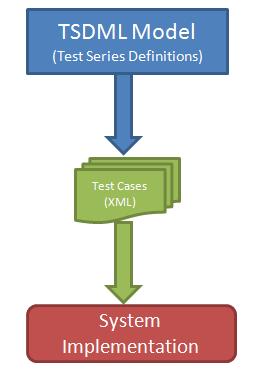
\includegraphics[width=0.35\textwidth]{figures/SystemRun.png}
	\caption{Test Cases Run on System Implementation}
	\label{fig:SystemRun}
\end{figure}


In the previous sections, an approach for modeling a system's behavior and structure from performance perspective was described. The approach described enabled generation of many test cases from TSDML models to be executed on a DEVS simulation engine running behavioral models of the system. There are two paths that can be taken from the model level to the system level:

\begin{itemize}
	\item Test cases may be executed on the real system (\ref{fig:SystemRun}). Running test cases on the real system for performance testing potentially gives the best results. However, this option may not always be available since it may be costly to run test cases with unpredictable outcomes on a real system. In such a case, it may be desirable to replicate the real system in a similar environment which may also be a costly operation. 
	\item Test cases may be executed on a simulation environment using behavioral models for the applications (\ref{fig:SimulationRun}). This path is less costly albeit the quality of performance test results are highly dependent on the quality of the system behavioral models.
\end{itemize}

\begin{figure}
	\centering
		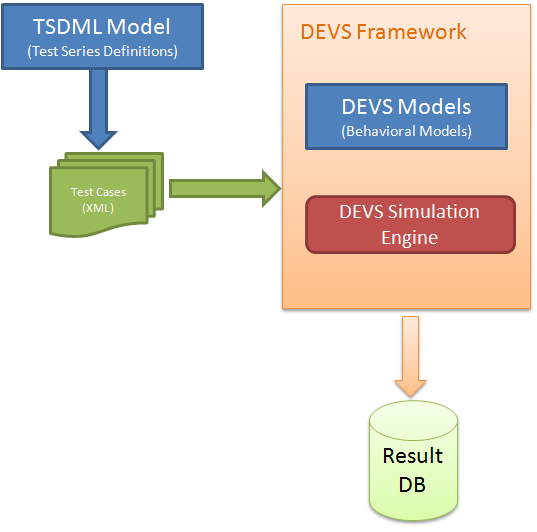
\includegraphics[width=0.40\textwidth]{figures/SimulationRun.png}
	\caption{Test Cases Run on Simulation Engine}
	\label{fig:SimulationRun}
\end{figure}

In either case mentioned above, there needs to be a way to make an assessment about the results of the test run. If performance requirements were clearly captured and each performance metric could be measured at the end of a test run, it might be possible to make pass/fail decision on the test run. However, the question is: is it desirable to merely verify performance, or in general non-functional requirements, in the same manner as functional requirements? One may argue that non-functional requirements testing phase in the development life cycle is more about observing, understanding how the system performs in different conditions, environments or with different system parameters. It is more valuable to be able to analyze test run results, reason about the system performance, and identify relationship of system parameters with performance then to make a pass/fail decision. From this perspective, (performance) testing approaches (performance) engineering. In this sense, it is crucial to be able to feed the results of a test run back into the system, thus closing the loop. This does not necessarily mean to automatically feed a test run result back into the system. This feedback may be in the form of understanding more about the system and devising more and interesting test cases with variations in system parameters or system environment. 

It is important to note that there is extensive literature on performance prediction from performance models and those literature was investigated in \cite{areapaper}. However, the approach described here is not about predicting the performance of a system from performance models as outline above. It is important to make the distinction between creating a performance model for a system and creating a system model and including a  performance aspect. In the approach described here, in a typical model based development sense, behavioral and structural abstractions of a system are captured in a system model and this model is extended from performance point of view. Since it is also possible to generate series of test cases from this system model, it is possible to run the actual test cases either on the real system or in a simulation environment to reason about the actual performance of the system.

\subsection{Performance Monitoring}
****TODO****

\subsection{Perturbation and Sensitivity Analysis}
Perturbation and sensitivity analysis methods that can be used to analyze results of a performance run. Using these techniques, one can observe the output of a system

-running the tests on the actual system automatically closes the loop
-performance engineering will give an idea about how the system performs
-not interested in prediction
-interested in what parameter change in the system cause what performance implication
-so far described test generation and execution. if tests run on real system, monitoring system performance will give information about the performance of the system. if tests run on simulation (in our case), need to measure and analyze the results to feed the findings back into the system. 
-design time performance analysis after simulation
-may reference from Prof. Karsai's monitoring book. Talk about monitoring but say we are interested in performance engineering.


\section{Summary}
****TODO****